%%%%%%%%%%%%%%%%%%%%%%%%%%%%%%%%%%%%%%%%%
% Beamer Presentation
% LaTeX Template
% Version 1.0 (10/11/12)
%
% This template has been downloaded from:
% http://www.LaTeXTemplates.com
%
% License:
% CC BY-NC-SA 3.0 (http://creativecommons.org/licenses/by-nc-sa/3.0/)
%
%%%%%%%%%%%%%%%%%%%%%%%%%%%%%%%%%%%%%%%%%

%----------------------------------------------------------------------------------------
%	PACKAGES AND THEMES
%----------------------------------------------------------------------------------------

\documentclass{beamer}

\mode<presentation> {

% The Beamer class comes with a number of default slide themes
% which change the colors and layouts of slides. Below this is a list
% of all the themes, uncomment each in turn to see what they look like.
%\usetheme{CambridgeUS}
%\usetheme{Copenhagen}
%\usetheme{Darmstadt}
%\usetheme{Dresden}
%\usetheme{Frankfurt}
%\usetheme{Goettingen}
%\usetheme{Hannover}
%\usetheme{Ilmenau}
%\usetheme{JuanLesPins}
%\usetheme{Luebeck}
%\usetheme{Madrid}
%\usetheme{Malmoe}
%\usetheme{Marburg}
\usetheme{Montpellier}
%\usetheme{PaloAlto}
%\usetheme{Pittsburgh}
%\usetheme{Rochester}
%\usetheme{Singapore}
%\usetheme{Szeged}
%\usetheme{Warsaw}

% As well as themes, the Beamer class has a number of color themes
% for any slide theme. Uncomment each of these in turn to see how it
% changes the colors of your current slide theme.

%\usecolortheme{albatross}
%\usecolortheme{beaver}
%\usecolortheme{beetle}
%\usecolortheme{crane}
%\usecolortheme{dolphin}
%\usecolortheme{dove}
%\usecolortheme{fly}
%\usecolortheme{lily}
%\usecolortheme{orchid}
%\usecolortheme{rose}
%\usecolortheme{seagull}
\usecolortheme{orchid}

%\setbeamertemplate{footline} % To remove the footer line in all slides uncomment this line
\setbeamertemplate{footline}[page number] % To replace the footer line in all slides with a simple slide count uncomment this line

\setbeamertemplate{navigation symbols}{} % To remove the navigation symbols from the bottom of all slides uncomment this line
}

\usepackage{graphicx} % Allows including images
\usepackage{booktabs} % Allows the use of \toprule, \midrule and \bottomrule in tables

%----------------------------------------------------------------------------------------
%	TITLE PAGE
%----------------------------------------------------------------------------------------

\title[AE471A ]{Parallel Proper Orthogonal Decomposition \\ Study and Implementation } % The short title appears at the bottom of every slide, the full title is only on the title page

\author{Govind Gopakumar} % Your name
\institute[IIT Kanpur] % Your institution as it will appear on the bottom of every slide, may be shorthand to save space
{
Indian Institute of Technology, Kanpur \\ % Your institution for the title page
\medskip
\textit{Roll number 11284} % Your email address
}
\date{\today} % Date, can be changed to a custom date

\begin{document}

\begin{frame}
\titlepage % Print the title page as the first slide
 \end{frame}

\begin{frame}
\frametitle{Overview} % Table of contents slide, comment this block out to remove it
\tableofcontents % Throughout your presentation, if you choose to use \section{} and \subsection{} commands, these will automatically be printed on this slide as an overview of your presentation
\end{frame}

%----------------------------------------------------------------------------------------
%	PRESENTATION SLIDES
%----------------------------------------------------------------------------------------

%------------------------------------------------
\section{Background}

\subsection{Proper Orthogonal Decomposition}

\begin{frame}
\frametitle{Proper Orthogonal Decomposition}
\begin{itemize}
\item
The Proper Orthogonal Decomposition - famous statistical procedure.\\ 
\item
Attempts to decompose a set of data into a different coordinate system, with the aim of compressing the data variance.
\item
Given a set of M x N data (M data points, N variables), it is possible to reduce to a set of M x P ( $ P \leq N$) with very low loss in accuracy.  
\end{itemize}
\end{frame}


\subsubsection{Theory}

\begin{frame}
\frametitle{Theory behind the POD}

\begin{itemize}
\item
Orthogonal linear transformation of dataset to new coordinate axis.
\item
New coordinate system such that first coordinate axis holds greatest variance of data, second holds second greatest, and so on.
\item
Projection of data is uncorrelated, and we can choose to ignore the latter axes. 
\end{itemize}

\end{frame}
% Sections can be created in order to organize your presentation into discrete blocks, all sections and subsections are automatically printed in the table of contents as an overview of the talk
%------------------------------------------------

\subsubsection{Applications}

\begin{frame}
\frametitle{Applications of POD}

\begin{itemize}
\item
In Computer Science, Statistics, and Data Analysis - Used for reducing dimensionality.
\item
Chaotic systems dynamics - Reduced order modelling enables easier computation of accurate solution.
\item
In Aerodynamics, POD helps characterise flows. POD modes can be used to generate flow models, up to reasonable accuracy.
\end{itemize}
\end{frame}


\subsubsection{Methods}

\begin{frame}
\frametitle{Computing the POD}
Suppose we have a set of data given by $x(t) \in R^n$ with $0 \leq t \leq T $. We seek a projection
$P_r : R^n \rightarrow R^r$ that minimises the total error \\

\begin{equation}
\int_0^T (||x(t) - P_r x(t)||)^2dt 
\label{pod:1}
\end{equation}

To solve this problem, we introduce the n x n matrix : 

\begin{equation}
R = \int_0^Tx(t)x(t)^*dt
\label{pod:2}
\end{equation}

where * denotes the transpose, and find the eigenvalues and eigen vectors of R, given by,

\begin{equation}
R\phi_k = \lambda_k \phi_k, \lambda_1 \geq \dots \geq \lambda_n \geq 0
\label{pod:3}
\end{equation}

\end{frame}

\begin{frame}
\frametitle{Computing the POD}
Since R is symmetric, positive-semidefinite, all the eigenvalues $\lambda_k$ are real and 
non-negative. The eigen values may be chosen to be orthonormal. This gives us an optimal 
subspace spanned by ${\phi_1, \dots, \phi_r}$ and the optimal projection given by:

\begin{equation}
P_r = \sum_{k=1}^r \phi_k \phi^*_k
\label{pod:4}
\end{equation}

The vectors $\phi_k$ are called POD modes.
\end{frame}


\subsubsection{Discrete version}
\begin{frame}
\frametitle{Eigenvalue based POD}
Easy way to understand in terms of data : 
\begin{itemize}
\item
The matrix we introduce captures the covariance of the data matrix.
\item
Computing the eigenvector decomposition of the matrix will capture the maximum variance.
\item
Ordering the eigenvectors by eigenvalues will order in decreasing variance.
\item
Equivalent to line fitting and dropping off-line terms in 2D.
\end{itemize}
\end{frame}

\begin{frame}
\frametitle{POD illustration}


\begin{figure}[H]
 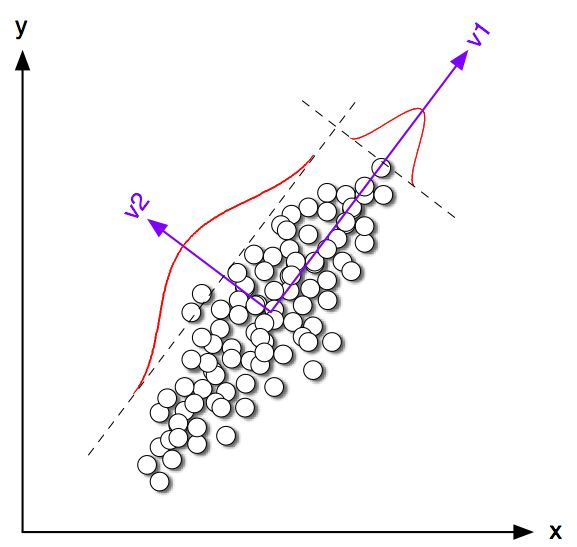
\includegraphics[scale=0.75]{pca_ex.jpg}
 \caption{POD illustration}
 \label{pod}
\end{figure}

\end{frame}


\subsection{CUDA}

\begin{frame}
\frametitle{Overview of CUDA}
CUDA : Compute Device Unified Architecture - This is NVIDIA corp.'s proprietary platform for parallel computation. \\
Advantages of CUDA over traditional parallel processing:
\begin{itemize}
\item
Hundreds of compute cores on a single device. 
\item
Massively parallelized architecture - heavily optimized for managing data and processes in parallel.
\item
Ideal for numerous small tasks.
\end{itemize}
\end{frame}

\subsubsection{Applications}

\begin{frame}
\frametitle{CUDA in Science}
Currently, popularity in scientific community is low, but it is extensively used in : 
\begin{itemize}
\item
Graphics rendering and computations
\item
Linear algebra routines
\item
Cryptography
\end{itemize}
\end{frame}

\subsubsection{Drawbacks}
\begin{frame}
\frametitle{Drawbacks with CUDA}
\begin{itemize}
\item
Accuracy - Double precision is relatively new.
\item
Power of a single node is relatively low
\item
Getting started is slightly tough.
\end{itemize}
\end{frame}

\section{POD on CUDA}
\subsection{Attempts so far}
\begin{frame}
\frametitle{Parallelizing the POD}

The state of the art is limited to the domain of computer science. The variant of POD, called Principal Component Analysis finds favour, and some work has been done on implementing it on GPUs.
\begin{itemize}
\item
Work has been done on multi-core implementations of the POD
\item
GPU processing is still in its infancy - very little work has been done.
\item
SVD - a related decomposition on GPU is a widely explored area.
\end{itemize}
\end{frame}
\subsection{Method followed}
\begin{frame}
\frametitle{Methodology}
\begin{itemize}
\item
CULA - A linear algebra library.
\item
Langauge agnostic - can be used in C++, C, Fortran
\item
Extensions to MATLAB, Python almost trivial
\item
Accelerated routines available commercially, at no cost to academics. 
\end{itemize}
\end{frame}

\section{Results}
\begin{frame}
Context : Three different kinds of results : 

\begin{itemize}
\item
Standard results published by CULA authors : NVIDIA C2070 GPU vs Intel Xeon X5660 hexa core
\item
HPCL PC : NVIDIA Quadro K2000 vs Intel Xeon E5-2690 20 core
\item
Consumer PC : NVIDIA GeForce GTX580 vs Intel Core i7 3770 quad core
\end{itemize}
\end{frame}
\subsection{Benchmarks}
\begin{frame}
\frametitle{Benchmarking}
Published benchmarks for eigenvector decomposition are available : 

\begin{figure}[H]
 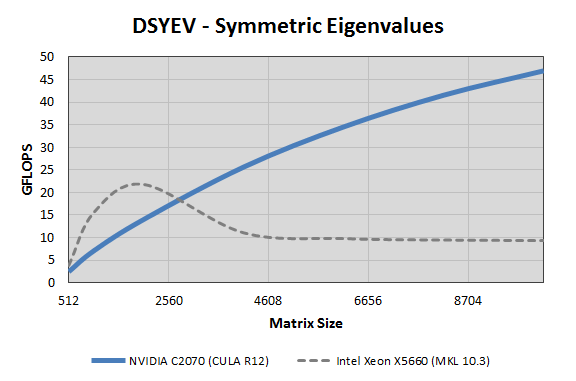
\includegraphics[scale=0.5]{DSYEV_N.png}
 \caption{Double precision Eigenvector decomposition - CULA}
 \label{dsyev}
\end{figure}
\end{frame}

\subsection{Real life results}
\begin{frame}
\frametitle{HPCL}
Actual results from simulations on HPCL PC:
\begin{figure}[H]
 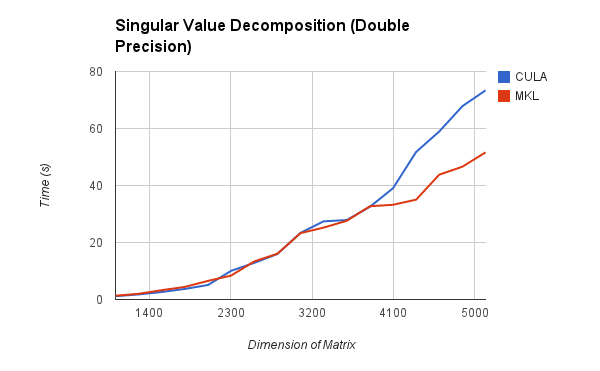
\includegraphics[width=\textwidth]{hpcldgesvd.png}
 \caption{Double precision SVD - HPCL}
 \label{hpcldgesvd}
\end{figure}
\end{frame}

\begin{frame}
\frametitle{Consumer PC}
Actual results from simulations on consumer PC:

\begin{figure}[H]
 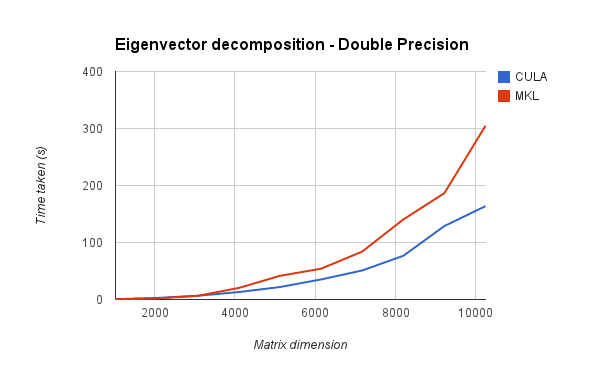
\includegraphics[width=\textwidth]{dsyev_bench.png}
 \caption{Eigenvector decomposition - Double precision benchmarks }
 \label{eigenbench}
\end{figure}

\end{frame}


\section{Conclusions}
\subsection{Inferences}
\begin{frame}
\frametitle{Inference from performance}

\begin{itemize}
\item
Performance of CPUs is easily matched, or even eclipsed by a standard GPU.
\item
Speed-ups offered can be almost 2x, depending on CPU vs GPU comparison.
\item
Accuracy is maintained till double precision.
\item
Results in case of highly polar configurations still show GPUs matching CPU speed.
\end{itemize}
\end{frame}

\subsection{Remarks}
\begin{frame}
\frametitle{Concluding remarks}
\begin{itemize}
\item
Compelling use case when applicable
\item
Specifically, POD speed can be increased up to two fold, with a good GPU based system.
\item
General linear algebra routines too can be accelerated
\item
Speed up achieved was using stock configurations, with optimizations, more than double the performance of normal CPUs can be reached.
\end{itemize}
\end{frame}

\section*{Questions}
%------------------------------------------------

%------------------------------------------------

\begin{frame}
\Huge{\centerline{The End}}
\end{frame}

%----------------------------------------------------------------------------------------

\end{document}